\chapter{总结和展望}\label{chap:6}

本论文切入光子集成芯片的痛点,迫切需要紧凑高性能的光子器件,用于降低较高的光子芯片成本。光子集成器件的设计往往具有较多的设计自由度、较复杂的器件需求和耗费时间的电磁波求解过程。因此需要运用高效可靠的算法来简化和加速器件设计和优化。

通过引入成熟可靠的有数十年研究的遗传算法,通过物竞天择适者生存的生物法则,实现了有效的变量优化,通过遗传算法,设计并优化了三个常用的光子集成器件。

在第三章中,提出并通过遗传算法设计了一种基于底部硅光栅反射镜的氮化硅光栅耦合器。通过下置式的硅光栅,实现较高的向上的辐射效率,从而极大的提升了器件的耦合效率。同时,又采用了一种便于制备的光栅一步刻蚀的方案,一方面保留了硅光栅反射镜的高效率,另一方面,避免了化学机械抛光CMP和高精度的电子束对准曝光HPA过程。并通过器件测试得到均匀光栅的耦合效率为-3.6dB和70nm的1dB带宽,而非均匀变迹光栅的耦合效率为-2.5dB和65nm的1dB带宽。设计的氮化硅光栅耦合器,性能突出,制备简单,在实际的器件制备和应用中具有较高的应用前景。
 
在第四章中,提出、设计、加工、测试了一种紧凑的10×5$\mu$m$^2$的超材料硅与氮化硅波导的层间耦合器,并创新性的采用了双层氮化硅的波导,在实现了稳定的硅-氮化硅层间耦合的情况下,又保证了足够大的层间间距。相比于传统的倒锥层间耦合器,具有紧凑高效率的特点。通过三维交叉结构来测试层间耦合器的性能,器件测试得到的三维交叉的插入损耗为-1.206dB@1531nm,即单个层间耦合器的损耗约为-0.6dB,且1dB带宽覆盖了所需要的1530-1570nm波段,通过这紧凑的三维层间耦合器,可以较好的满足密集的三维层间耦合应用的需求。

在第五章中,设计并加工了一个紧凑的超材料长通滤波器,器件尺寸仅为5.1×5.1$\mu$m$^2$。在长通滤波器的长通波段(1550-1600nm),器件的插入损耗仅为-0.58dB。而在短波长截止波段(约1450-1500nm),光会由于超材料结构的电磁响应而被过滤并反射,且功率衰减可以达到25dB。同样,展示了长通滤波器的由于器件版图缩放导致的过渡带偏移现象和由器件级联带来的过渡带斜率增强现象。这些实验结果表明,超材料可以成为一种紧凑而理想的设计方法,用来实现片上的滤波功能,对于提高光子器件的集成度和降低光子集成芯片成本,具有积极的意义。

\begin{figure}[!htbp]
    \centering
    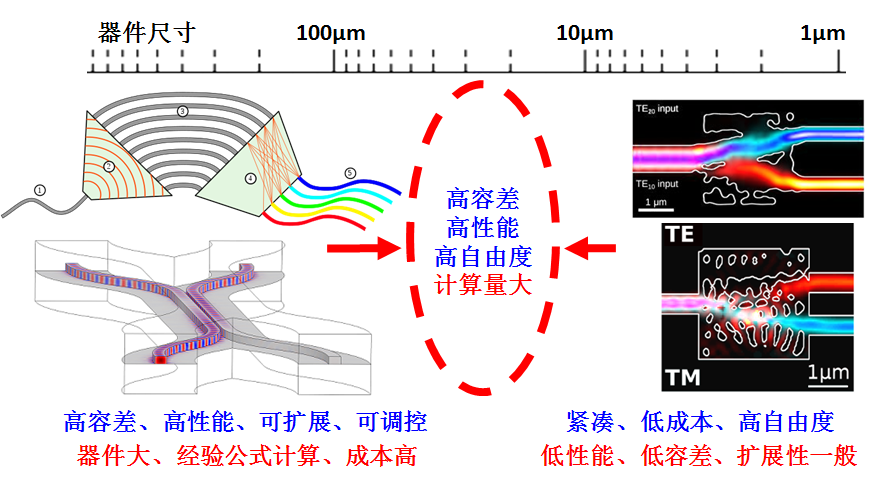
\includegraphics[width=1\textwidth]{Img/6-2.png}
    \caption{传统的光子集成器件,器件尺寸较大($>$100$\mu m$),具有更高的性能等优点;数值计算的光子集成器件,器件尺寸非常小($<$10$\mu m$),则性能较为一般。}
    \label{fig:6-2}
\end{figure}
%%%%%%%%%%%%%%%%%%%%%%%%%%%%%%%%%%%%%%%%%%%%%%%%%%%%%%%%%%%%%%%%%%%%%%%%%%%%%%%%%%%%%%%%%%%%%%%%%%%%%%%%%%%%

如图6.1所示,传统应用的光子集成器件,器件尺寸较大($>$100$\mu m$),具有较高的性能、较好的器件容差特性,可拓展、可调控等优点。
而较大的器件尺寸,依赖经验公式或近似方法等低自由度的方法进行器件设计,自由度较低,较大的器件尺寸也提高了光子芯片的制造成本,不利于光子芯片的大规模应用。
另一方面,通过数值优化算法计算的到光子器件,器件尺寸小($<$10$\mu m$),具有极高的紧凑性和集成度,可通过极高的自由度,实现更多样的性能;
而,器件的尺寸小(目前发表的基于计算的光子器件,尺寸往往在$<$5$\mu m$),性能较低,容差较差,器件的拓展性一般。
因此,在10$\mu m\sim$100$\mu m$的器件尺寸范围内,存在一个兼顾高自由度,高性能、高容差的器件设计尺寸范围。数十微米的器件尺寸下的高自由度器件设计,需要耗费宏大的计算机资源,对数值优化算法是一种巨大的挑战。遗传算法将在大规模的光子器件设计优化中,发挥更加重要的作用。